% This must be in the first 5 lines to tell arXiv to use pdfLaTeX, which is strongly recommended.
\pdfoutput=1
% In particular, the hyperref package requires pdfLaTeX in order to break URLs across lines.

\documentclass[11pt]{article}

% Remove the "review" option to generate the final version.
\usepackage[final]{acl}

% Standard package includes
\usepackage{times}
\usepackage{latexsym}

% For proper rendering and hyphenation of words containing Latin characters (including in bib files)
\usepackage[T1]{fontenc}
% For Vietnamese characters
% \usepackage[T5]{fontenc}
% See https://www.latex-project.org/help/documentation/encguide.pdf for other character sets

% This assumes your files are encoded as UTF8
\usepackage[utf8]{inputenc}

% This is not strictly necessary, and may be commented out,
% but it will improve the layout of the manuscript,
% and will typically save some space.
\usepackage{microtype}

\usepackage{graphicx}


% If the title and author information does not fit in the area allocated, uncomment the following
%
%\setlength\titlebox{<dim>}
%
% and set <dim> to something 5cm or larger.

\title{Tuning and Interpreting BERT for Patronizing and Condescending Language}

% Author information can be set in various styles:
% For several authors from the same institution:
% \author{Author 1 \and ... \and Author n \\
%         Address line \\ ... \\ Address line}
% if the names do not fit well on one line use
%         Author 1 \\ {\bf Author 2} \\ ... \\ {\bf Author n} \\
% For authors from different institutions:
% \author{Author 1 \\ Address line \\  ... \\ Address line
%         \And  ... \And
%         Author n \\ Address line \\ ... \\ Address line}
% To start a seperate ``row'' of authors use \AND, as in
% \author{Author 1 \\ Address line \\  ... \\ Address line
%         \AND
%         Author 2 \\ Address line \\ ... \\ Address line \And
%         Author 3 \\ Address line \\ ... \\ Address line}

\author{Thomas Gao \\
  University of California, Berkeley \\
  \texttt{tgao2020@berkeley.edu} \\}

\begin{document}
\maketitle
\begin{abstract}
In support of SemEval-2022 Task 4, Patronizing and Condescending Language (PCL) Detection, we present a fine-tuned BERT model for identifying PCL embedded in news articles, which meaningfully outperforms baseline models with an F1-score of 0.52. We apply the Integrated Gradients method to attribute the model’s prediction to individual words, thereby revealing the learned knowledge of the model. We found that the model encodes explicit PCL vocabulary well, but has bias for racial and religious terms. The model falls short of truly understanding PCL, struggling to differentiate factual statements and PCL and capturing PCL without explicit words.
\end{abstract}

\section{Introduction}

Patronizing and Condescending Language (PCL) is language use that shows a discourse of pity and superior attitudes towards others. PCL usage in general media, while often well-intentioned, might nevertheless routinize discrimination and lead to greater inequalities~\cite{perez2020don}.

In SemEval-2022 Task 4: Patronizing and Condescending Language Detection, the organizers created the Don’t Patronize Me! dataset, which contains over 10,000 paragraphs about vulnerable communities extracted from news stories. The dataset has been annotated to indicate the presence of PCL, categories of PCL and corresponding text spans. Our research focuses on subtask 1, which is to predict the presence of PCL as a binary classification problem.

To address this problem, we experiment with Logistic Regression with the bag-of-words model, CNN with Global Vectors for Word Representation (GloVe)~\cite{pennington2014glove}, and Bidirectional Encoder Representation from Transformer (BERT)~\cite{devlin2018bert}. Our up-sampled BERT model yields an F1-score of 0.52, meaningfully better than the baseline models. For the BERT model, we use Integrated Gradients~\cite{sundararajan2017axiomatic} to shed light on the model knowledge and mistakes, which can be used as pointers for future research. 

In the rest of this paper, we organize the content as follows: related work of harmful language modeling in section 2; section 3 introduces data description, preprocessing, and model methodologies; section 4 discusses experimental results; section 5 presents sample model predictions and their attributions; section 6 discusses interesting areas for future work. We also present the conclusion of our work at the end of the paper.


\section{Related Work}

There were similar tasks aimed at studying harmful languages. In SemEval 2019 Task 6 Identifying and Categorizing Offensive Language~\cite{zampieri2019semeval}, models used ranged from traditional machine learning, e.g. SVM and logistic regression, to deep learning, e.g. CNN, RNN, BiLSTM, ELMo and BERT. Among the top-10 teams, seven used BERT. For the classification task, the top team experimented with different models including linear models and LSTM, and found pre-trained BERT with fine-tuning performed best. The runner-up team also used BERT model and applied techniques to address the class imbalance in the training data.

Compared to offensive language, patronizing language in news articles is more challenging to model because of the subtlety. However, the organizers show that BERT-based approaches show non-trivial results and outperform simpler models~\cite{perez2020don}. A review of submitted papers for the task show that the top performing team PALI-NLP uses a novel Transformer-based model BERT-PCL with two discriminative fine-tuning strategies~\cite{hu2022pali}, and another team achieving top quartile performance ensembles five RoBERTa models that are seeded differently~\cite{zhao2022utsa}. Team SATLab uses a logistic regression model only fed with characters and word n-grams and obtained performance lower than the best teams~\cite{bestgen2022satlab}.

Our work therefore studies the BERT-based models. Specifically, we fine-tune the BERT model to reproduce the meaningful results and use Integrated Gradients~\cite{sundararajan2017axiomatic} method to analyse BERT's learned knowledge and predictions.

\section{Data and Methodology}

\subsection{Data Description}

The Don’t Patronize Me! Dataset includes paragraphs about vulnerable communities extracted from news stories from the News on Web (NoW) corpus~\cite{davies2013corpus}. Articles with at least one word from a list of selected keywords, e.g. disabled, homeless, women, vulnerable, were split into paragraphs and then randomly selected.

The data was annotated by three annotators, with two annotators annotating the whole dataset and the third one acting as a referee to provide a final label in case of disagreement. In the first step, annotators determined which paragraphs contain PCL. In the second step, the annotators indicate, in paragraphs containing PCL, the text span of PCL and its category. Out of the seven categories, the most common ones are Unbalanced Power, Compassion, and Presupposition.

The organizer created an 80/20 split of the training dataset. The dataset distribution is summarized in Table~\ref{tab:dist}. They also reserved 3897 paragraphs for scoring. From the table, we observe class imbalance with the vast majority of paragraphs not containing PCL.

\begin{table}
\centering
\begin{tabular}{lccc}
\hline
\textbf{Data} & \textbf{Train} & \textbf{Dev} & \textbf{Total} \\
\hline
Paragraphs & 8375 & 2094 & 10469  \\
PCL(\#) & 794 & 119 & 993  \\
\hline
PCL(\%) & 9.48\% & 9.50\% & 9.49\% \\
\hline
\end{tabular}
\caption{Data distribution: class imbalance with most text not including PCL.}
\label{tab:dist}
\end{table}

Regarding the text span annotation and PCL categorization, it is worth noting that between the two annotators, there are 1359 instances of agreement and 1401 instances of misalignment, demonstrating the subjective nature of PCL.


\subsection{Preprocessing}

\textbf{Data imbalance}  In order to create a more balanced training dataset, we reduce the number of paragraphs without PCL to the first 1588 paragraphs, i.e. twice the number of paragraphs with PCL. This gives us 2382 training examples, of which 794 contain PCL. We also create an upsampled dataset by duplicating the minority class 5 times, creating a dataset with 11551 training examples, of which 3970 contain PCL, which is used to train the final BERT model.


\subsection{Methodology}

\textbf{Epoch} We train our deep learning models for 3-5 epochs and select the epoch that produces the highest F1-score on the dev dataset. We also monitor the validation loss and consider only epochs before validation loss rising to avoid overfitting.

\textbf{Logistic Regression}  We use CountVectorizer from scikit-learn library to transform text into features. Then, we fit Logistic Regression as our baseline model to determine the baseline performance. 

\textbf{CNN with GloVe}  We use 300-dimensional word embeddings from GloVe~\cite{pennington2014glove} to represent the text, and train single-channel CNN with 128 filters, kernel size of 5, stride of 1, 256 hidden units and L2 regularization of 1e-05. 

\textbf{BERT}  BERT model~\cite{devlin2018bert} uses Transformer architecture~\cite{vaswani2017attention} and pretrains on a massive amount of texts to learn context-aware word embeddings and sentence embeddings. We download the pre-trained \textit{bert-base-cased} model from Hugging Face and fine-tune the model by attaching a dense layer of 256 hidden nodes to the sentence embedding vector, i.e. [CLS] token embedding. We then include a dropout layer with a dropout rate of 0.1 before making a prediction with the sigmoid activation function. We use binary cross entropy loss, Adam optimizer with a learning rate of 5e-5 and max length of 128 words and train all layers.

\section{Experiment Results}

The official evaluation metric of this task is the F1-score of the positive class. Predicting the majority class, i.e. no PCL, would produce F1-score of 0 because recall is 0. Random guess would F1-score of 0.1604.

Our machine learning models all perform better than random guesses, with the BERT models producing meaningfully better results than Logistic Regression (BOW) and CNN (GloVe). The upsampled model produces a higher F1-score than the downsampled model, as expected given more data. We submitted our predictions on the test data reserved by the organizers, and achieved an F1-score of 0.5068, slightly lower than the score on the dev dataset. See table ~\ref{tab:perf} for model performance.


\begin{table*}
\centering
\begin{tabular}{lcccc}
\hline
\textbf{Model} & \textbf{Epochs} & \textbf{Precision} & \textbf{Recall} & \textbf{F1} \\
\hline
Random & NA & 0.0955 & 0.5000 & 0.1604  \\
Logistic Regression (BOW) & NA & 0.2588 & 0.4824 & 0.3368  \\
CNN (GloVe) & 2 & 0.3127 & 0.4824 & 0.3794  \\
BERT (Down Sampled) & 1 & 0.3537 & 0.7286 & 0.4762  \\
BERT (Up Sampled) & 1 & 0.5464 & 0.5022 & \textbf{0.5236}  \\
\hline
\end{tabular}
\caption{Model Performance for PCL Classification on Dev Data.}
\label{tab:perf}
\end{table*}

\section{Model Interpretation}

To understand how the BERT model is making the predictions, we examine the contribution of each word to the overall prediction using the Integrated Gradients method~\cite{sundararajan2017axiomatic}. 

For feature embedding, we use the BERT input embedding; for baseline embedding, we use zero embedding for word tokens and BERT input embedding for non-word tokens. Between the input word embedding and baseline word embedding, we create 40 equally spaced embedding steps. We record the gradients of the final prediction with respect to the input values at each embedding step, and compute the attribution of each word by summing the products of gradients and step embedding.

Figure~\ref{fig:fig1} shows top examples where the model is most confident. We attribute the model predictions to words, with green and red backgrounds indicating positive and negative contribution to PCL prediction and the darkness of colors corresponding to the magnitude of the contribution. We also use the span annotations where the two annotators are in agreement as the gold span, colored in orange, and provide the PCL category. Additional examples are included in the appendix~\ref{sec:appendix}.

\begin{figure*}
    \centering
    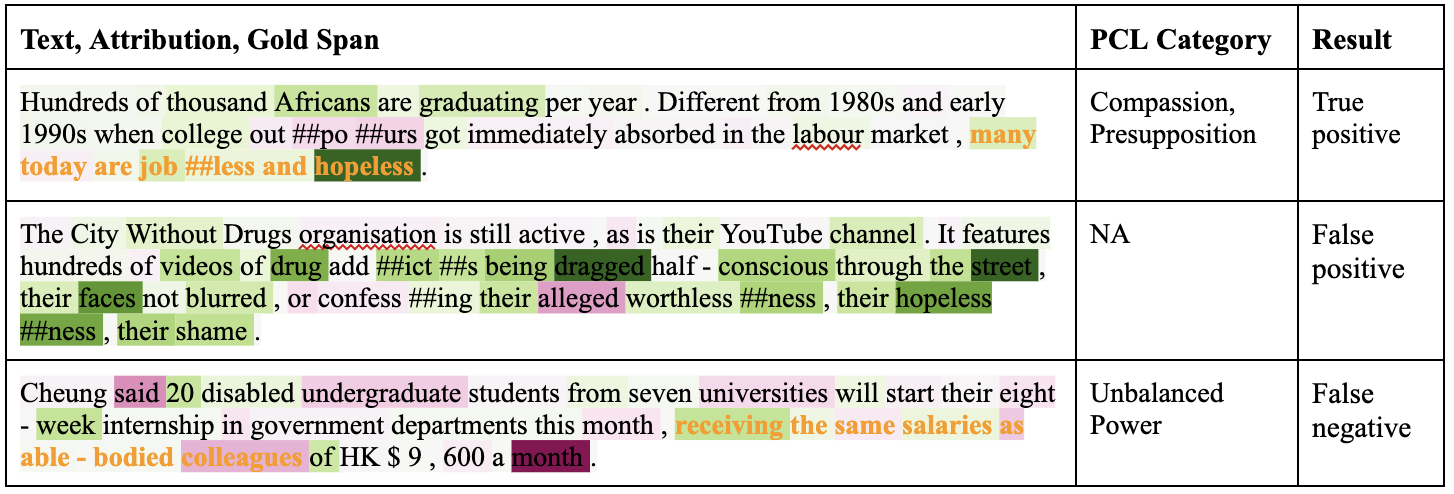
\includegraphics[width=16cm]{Fig 1.png}
    \caption{True Positive, False Positive and False Negative Examples with Highest Confidence}
    \label{fig:fig1}
\end{figure*}

In the first example, annotators consider the sentence to contain PCL because of presupposition and compassion. Presupposition assumes a situation as certain without having all the information. Compassion presents the vulnerable people as needy, raising a feeling of pity. Our judgment is that both PCL categories refer to the word \textit{hopeless}. From the green highlights, we see that the model rightly considers \textit{hopeless} as the main PCL driver. We also see that the word \textit{Africans} is assigned a green color, raising concern about racial bias in the data and the model.

In the second example, the model predicts positive class confidently based on the description of the videos. The subjects are described as being in a completely wretched and helpless state and words such as \textit{dragged}, \textit{worthlessness}, \textit{hopelessness} are highlighted as main contributors. However, the annotators judged that these are not PCL, and we concur because these words show up in a factual statement about the videos. The model expertly observed relevant words but failed to understand the nuance between facts and PCL.

The third example does not contain explicit PCL words. The model predicts false on the basis of \textit{month}, \textit{said}, \textit{undergraduate}, \textit{universities}, \textit{colleagues}. The first two are neutral vocabularies while the latter three words might be associated with capability and enablement. The annotators categorized this as Unbalanced Power most likely due to the intentional comparison between able-bodied and disabled students. We agree that the language would cause harm to the disabled community, and it is an example of implicit PCL.

In summary, our model is capable of making note of vocabularies that are likely to be associated with PCL. However, as shown in our examples, presence of such words does not automatically mean PCL, and PCL can also be implicit and not contain any explicit PCL words. In appendix~\ref{sec:appendix}, we also observe that vulnerable and religious vocabularies are associated with PCL, leading to false positive predictions. On the other hand, certain seemingly innocent words, e.g. \textit{administration}, can sometimes dominate in false negative predictions. This might be due to overfitting and supports the case of ensembling.

\section{Future Work}

Due to time limitations, there are additional architectures that we would like to experiment with. One such task is to explore multi-objective learning by including an additional training objective of PCL span detection using the annotated span data. We expect that by highlighting the specific text spans that contain PCL, the model can gain more accurate understanding and achieve better prediction. The study would also reveal the usefulness of highlighting text span in addition to assigning binary labels when annotating data.

\section{Conclusion}

In this paper, we explore how pre-trained BERT models can be fine-tuned for classifying whether a paragraph contains PCL. This standard approach achieves an F1-score of 0.52, a non-trivial result compared to baselines. 

We also use the Integrated Gradients method to attribute the model’s decisions and gain insights into the model’s learned knowledge. We find that the model encodes explicit PCL vocabulary well, but falls short on differentiating between facts and PCL and capturing PCL without explicit words. We also find evidence of racial and religious bias in the model.

PCL is harmful but often unconscious language use due to a lack of perspectives of the vulnerable communities. Machine learning has a great opportunity to encode perspectives from vulnerable communities and reduce such harmful language use in our society.

\section*{Acknowledgements}

We would like to thank Joachim Rahmfeld for his guidance and feedback. We are also grateful to the W266 faculties for their wonderful teaching through live sessions, notebooks and paper reading sessions. The authors are responsible for any errors that remain.

% Entries for the entire Anthology, followed by custom entries
\bibliography{anthology,custom}

\appendix

\section*{Appendix: Additional Examples}
Figure~\ref{fig:fig2} below shows additional examples of classification attribution. 

\label{sec:appendix}

\begin{figure*}[t]
    \centering
    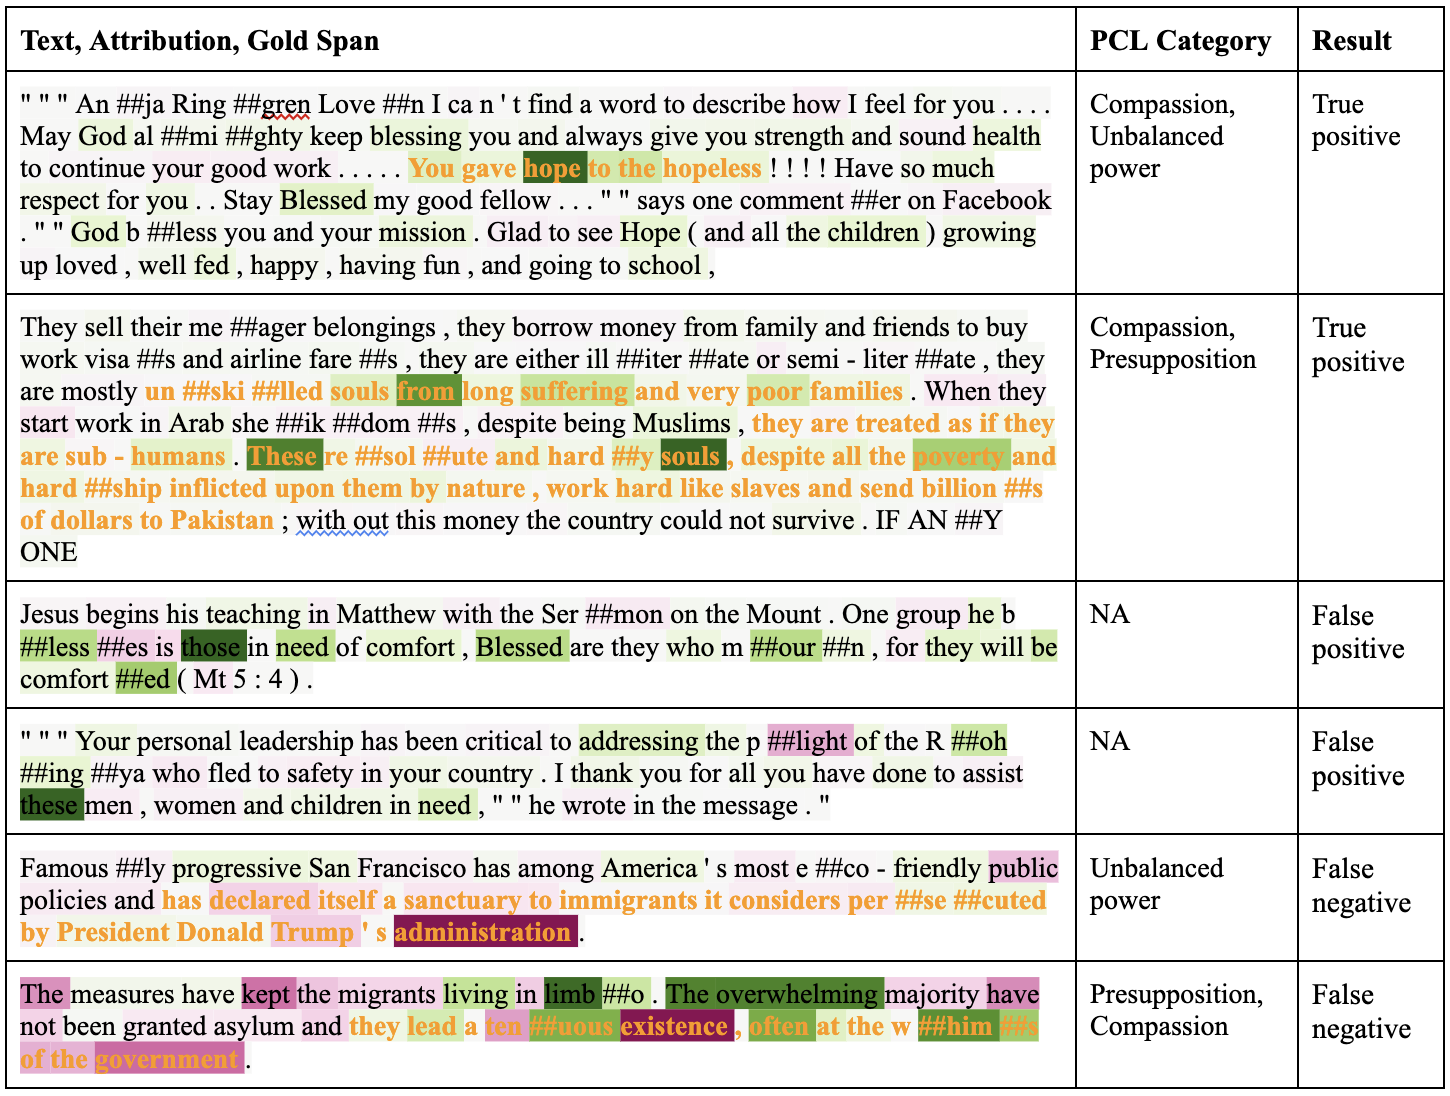
\includegraphics[width=16cm]{Fig 2.png}
    \caption{True Positive, False Positive and False Negative Examples with Highest Confidence}
    \label{fig:fig2}
\end{figure*}

\end{document}
